\newpage
\appendix

\section{Supporting Analysis for Scenario Sampling}
\label{app:scenario_sampling}

This appendix provides supporting evidence for the choice to sample the planned duration error in the scenario generation procedure.

The planned duration is compared with the historical average realized duration per surgery type. For both estimators, the sum of absolute errors with respect to the realized duration is computed. The results are shown in Table~\ref{tab:absolute_errors}.

\begin{table}[h]
    \centering
    \caption{Comparison of sum of absolute errors}
    \label{tab:absolute_errors}
    \begin{tabular}{l r}
        \hline
        Estimator & Sum of abs. errors in minutes \\
        \hline
        Planned duration & 333{,}179 \\
        Avg. realized duration per surgery type & 375{,}746.81 \\
        \hline
    \end{tabular}
\end{table}

The sum of absolute errors when using the historical average realized duration per surgery type equals $112.8\%$ of the sum of absolute errors obtained when using the planned duration. Therefore, the error is $12.8\%$ higher when using the historical average realized duration instead of the planned duration.

Figures~\ref{fig:hist_average_realized_error} and~\ref{fig:hist_planned_duration_error} show the corresponding error distributions.

\begin{figure}[h]
    \centering
    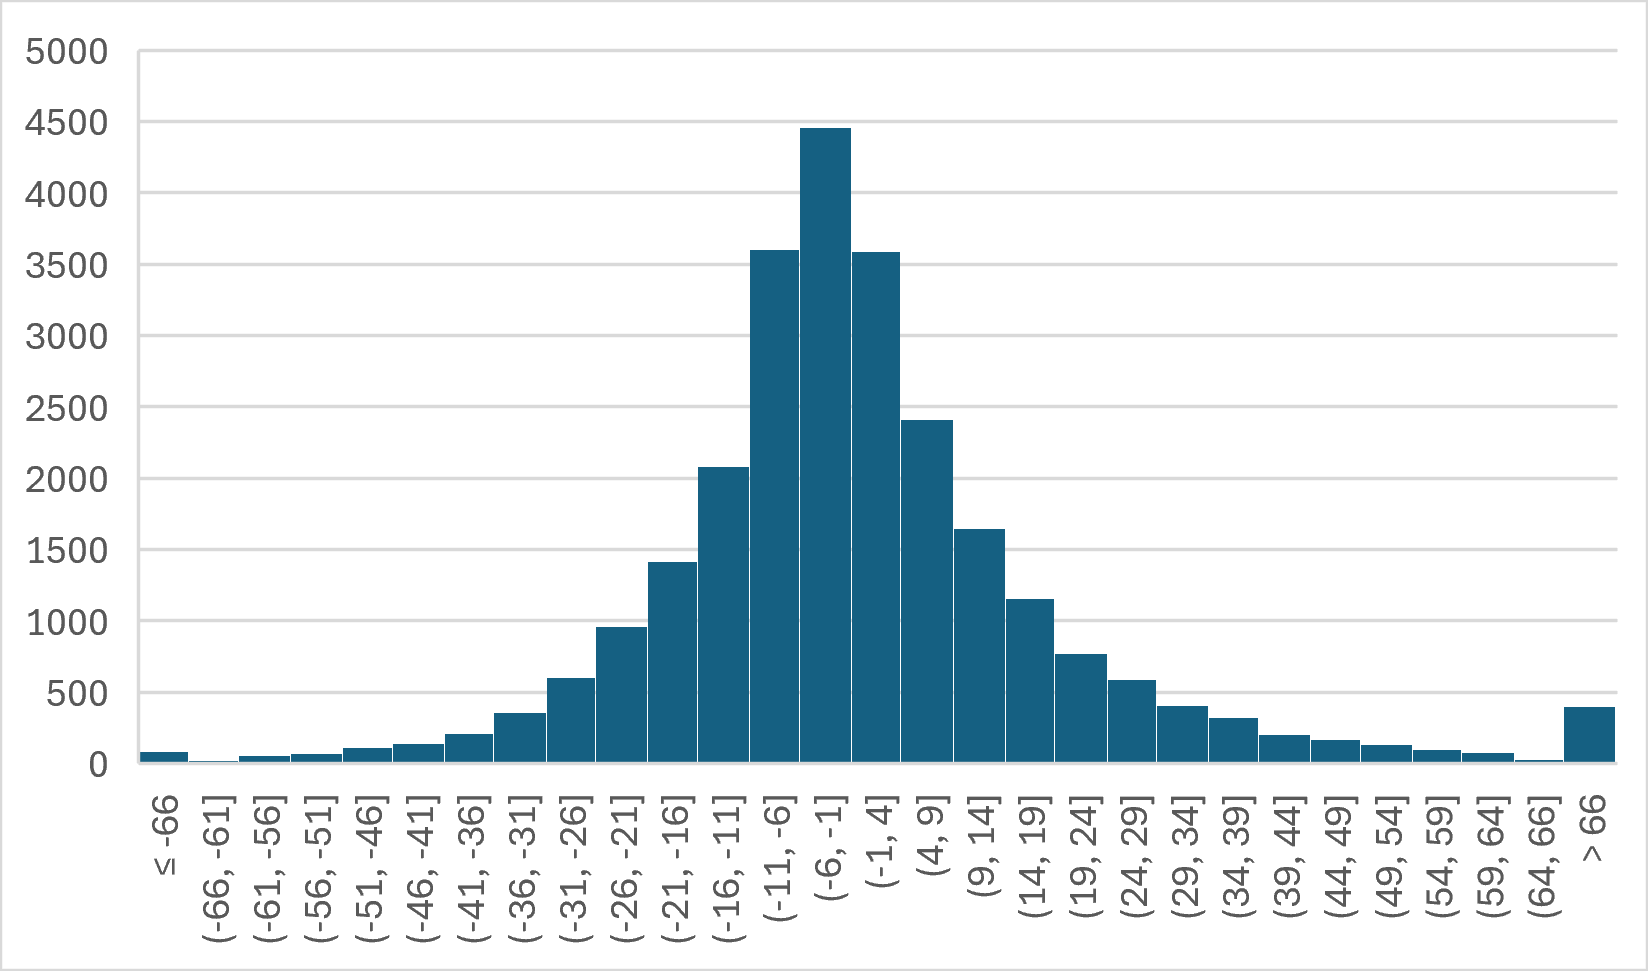
\includegraphics[width=1\linewidth]{Figures/histogram_average_realized_error.png}
    \caption{Histogram of the prediction error when using the historical average realized duration per surgery type.}
    \label{fig:hist_average_realized_error}
\end{figure}

\begin{figure}[h]
    \centering
    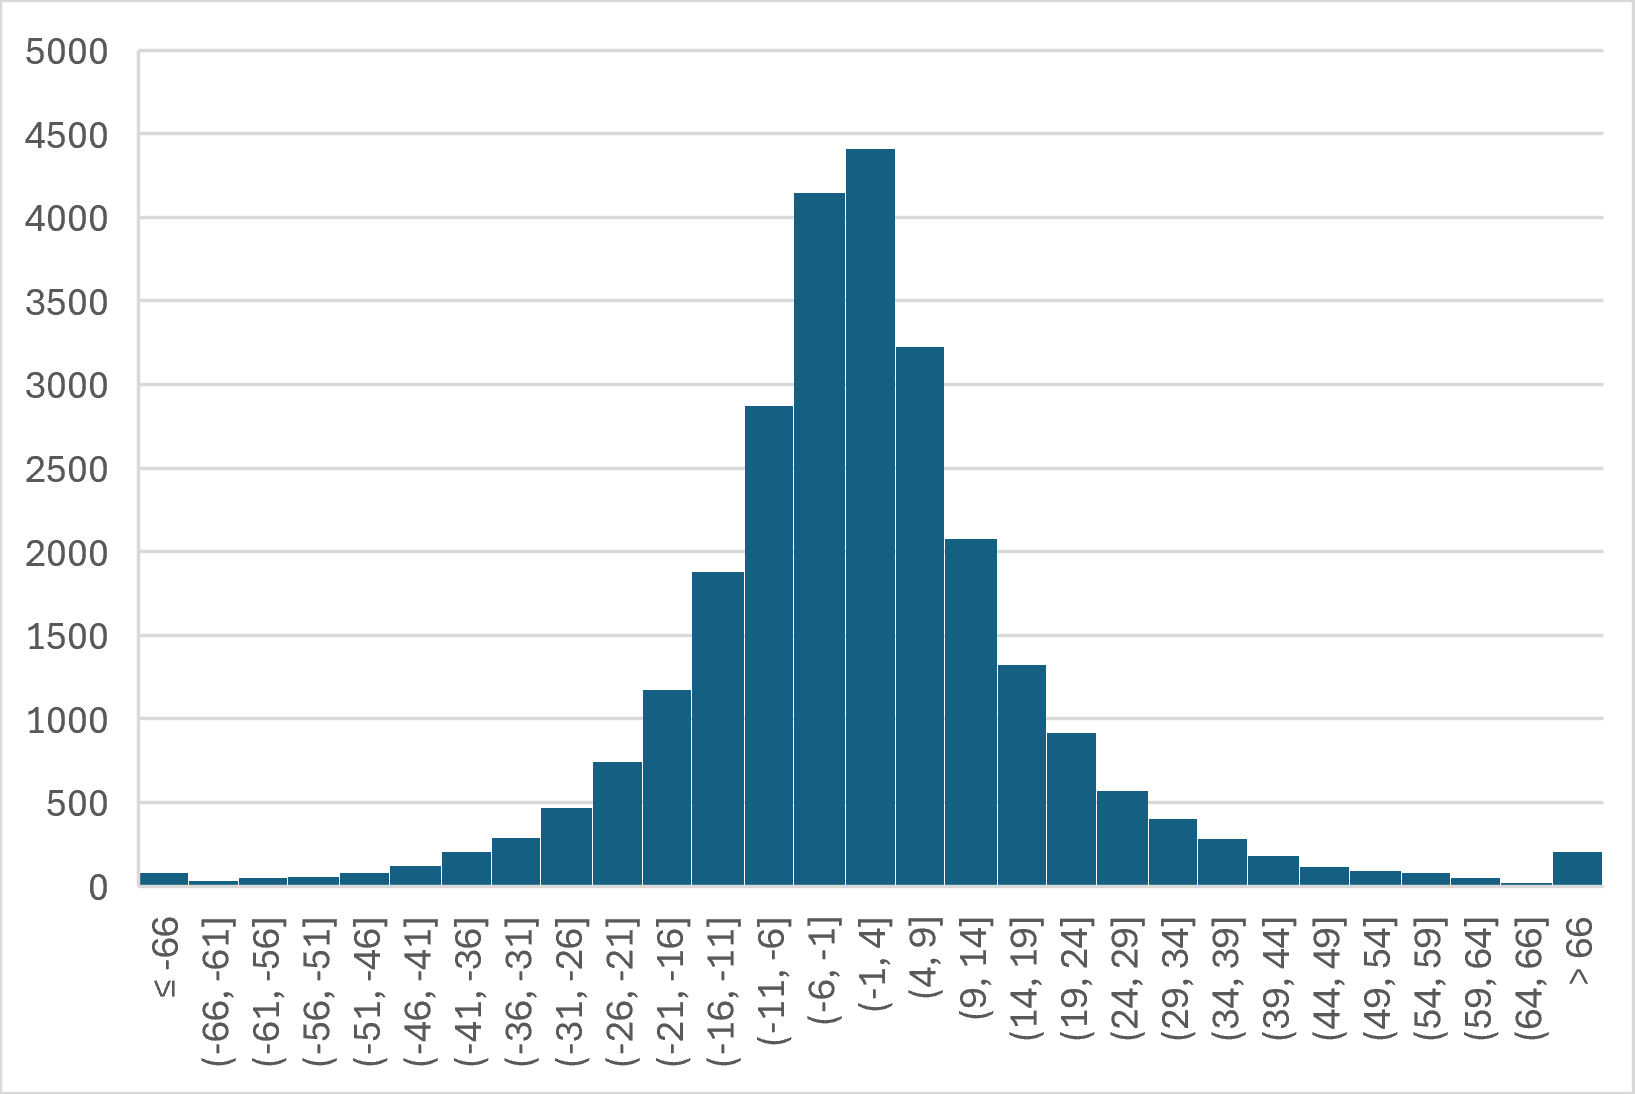
\includegraphics[width=1\linewidth]{Figures/histogram_planned_duration_error.png}
    \caption{Histogram of the prediction error when using the planned duration.}
    \label{fig:hist_planned_duration_error}
\end{figure}